\documentclass[12pt letterpaper]{article}

\usepackage{fullpage}
\usepackage{graphicx}
\usepackage{amsmath}

\providecommand{\e}[1]{\ensuremath{\times 10^{#1}}}
\usepackage{gensymb}

\usepackage{float}


\title{Gamma Ray Spectroscopy}
\author{Johnny Minor \\ Partner: Kayla Mitchell}
\date{\today}

\begin{document}

\maketitle

%abstract should have a very brief overiew of the goals and main results of the experiment. 
\begin{abstract}
In this experiment we used given data to study the gamma ray interactions of various radioactive sources. The radiation comes from a decay of a nucleus which then interacts with a NaI crystal scintillator that would then register the data. Unfortunately the equipment was broken so we used data from previous classes. We used the software Origin to make plots of the channel number versus counts. We then created a calibration plot which allowed us to create a map from channel number to energy. We then were able to analyze each element for it's various mechanisms of interaction such as the photoelectric effect, the Compton effect, back scattering, and beta spectrum. We also attempted to calculate the rest mass of the electron and analyze an unknown sample. 
\end{abstract}

\newpage

\section*{Description of Experiment}

We were not able to actually conduct an experiment due to the equipment being broken. We instead used data from previous year students. However, it might still be good to explain the apparatus for gamma ray spectroscopy. 

The apparatus we would have used would be very similar to the one found in the figure \ref{fig:scintillator}. We would have had our seven radioactive sources that we would have swapped out and recorded the gamma ray spectrum. 

\begin{figure}[H]
  \caption{Schematic of a scintillation counter.}
  \centering
    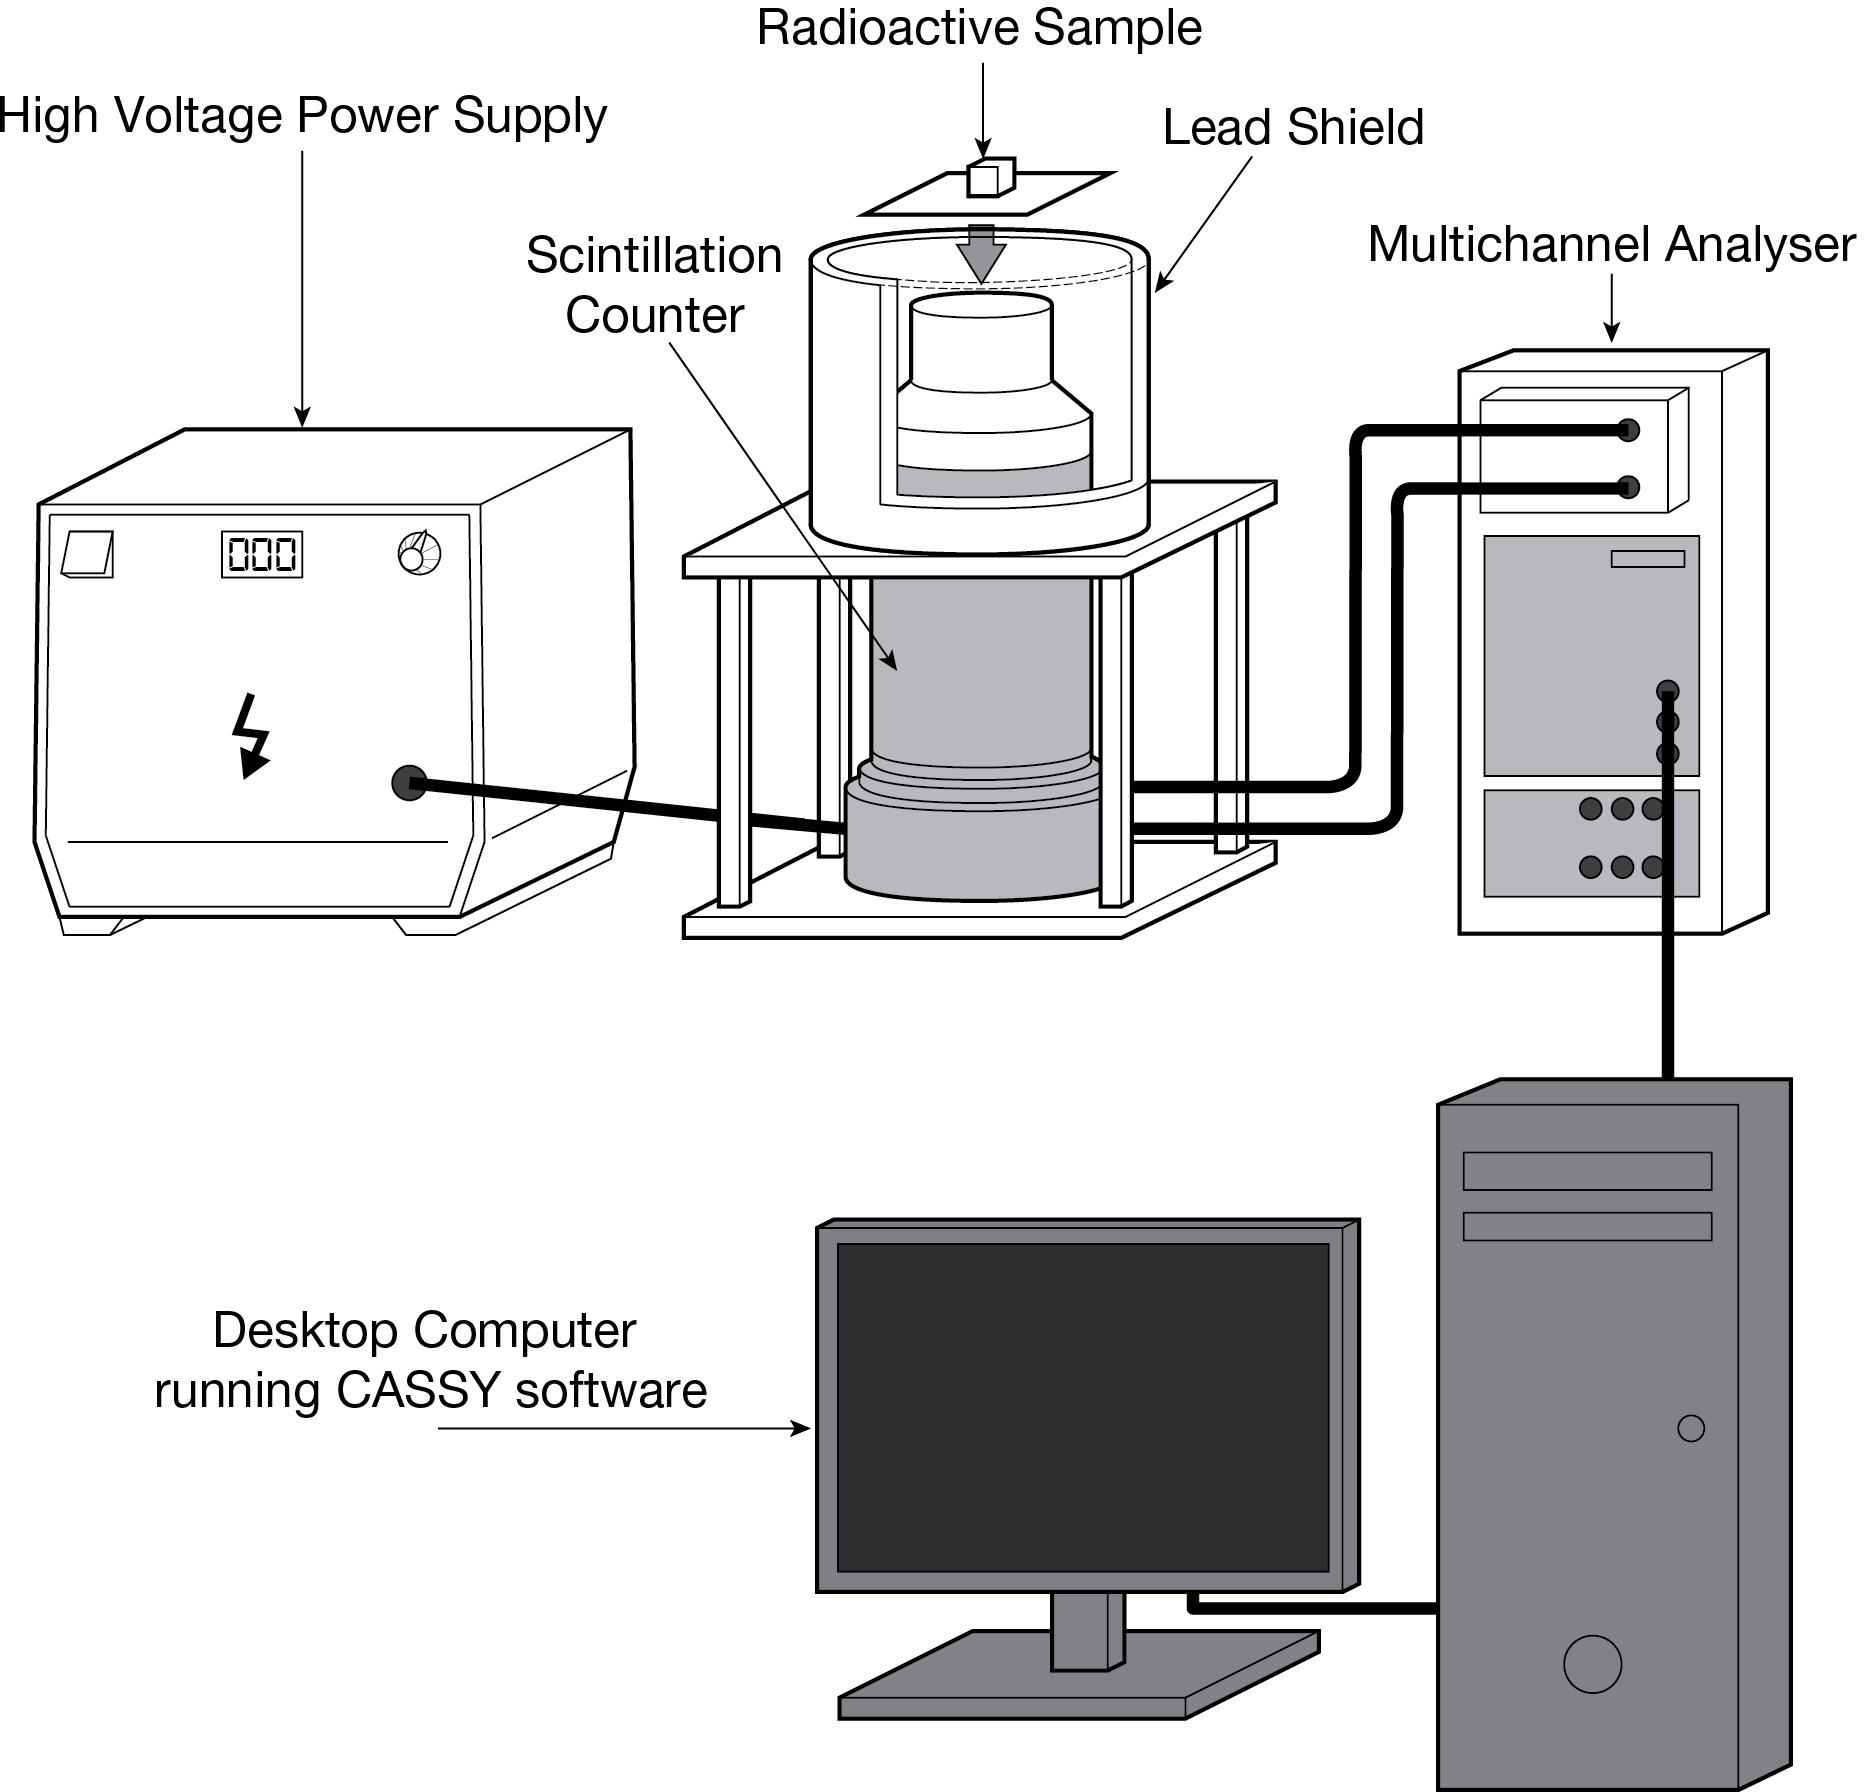
\includegraphics[width=.5\textwidth]{scint_spec.jpg}
    \label{fig:scintillator}
\end{figure}


When the radioactive source is placed in front of the NaI(Tl) scintillator the gamma ray will enter the scintillator and will interact with the NaI crystal. The crystal will emit light that corresponds to how much energy the gamma ray had when it interacted with the crystal. This light will then go through a photomultiplier and finally will be recorded with it's channel number. This can then be made into a histogram. In our scenario this bin versus number of counts was given to us.  

This is all the physics that was involved and the rest of the experiment was in the analysis of the gamma ray spectrum of the elements that we were given. 

\section*{Data and Analysis}

Once the bin versus number of counts histogram had been created for all of the elements we would then go on to create a calibration plot. We would fit a local Gaussian distribution on each elements photo peak because this is what were told by Dr. Engels. It can be motivated because the photo peak looks to be Gaussian by inspection. This fit allowed us to find what bin the peak was. We then found the energy that this corresponded to in the literature. Our calculations and findings can be seen in table \ref{calibration_table}. 

\begin{table}[H]
\centering
\caption{The data of photo peak channel and the value found in literature.}
\label{calibration_table}
\begin{tabular}{|l|l|l|}
\hline
Element & Channel & \begin{tabular}[c]{@{}l@{}}Photo Peak \\ (MeV)\end{tabular} \\ \hline
Am241   & 27.767  & 0.05936                                                     \\ \hline
Ba133   & 140.60  & 0.356                                                       \\ \hline
Cd109   & 40.025  & 0.08804                                                     \\ \hline
Co57    & 54.005  & 0.12206                                                     \\ \hline
Co60    & 330.99  & 1.17321                                                     \\ \hline
Co60    & 451.60  & 1.33247                                                     \\ \hline
Cs137   & 262.26  & 0.66164                                                     \\ \hline
Mn54    & 327.76  & 0.83403                                                     \\ \hline
Na22    & 482.97  & 1.2745                                                      \\ \hline
\end{tabular}
\end{table}

We then plotted these values as a scatter plot and then fit a linear equation to the scatter plot. This is motivated by inspection of the scatter plot (figure \ref{fig:calibration}) clearly showing a linear trend. We found the linear equation to be 

\begin{equation}
y = -0.02838 + 0.00291 x.
\end{equation}

This equation then allowed use to create a linear map from our channel to an actual energy. So we were able to create our new values of energy with this equation using $x$ values between 0 and 3000 with spacing of one. 

\begin{figure}[H]
  \caption{Schematic of a scintillation counter.}
  \centering
    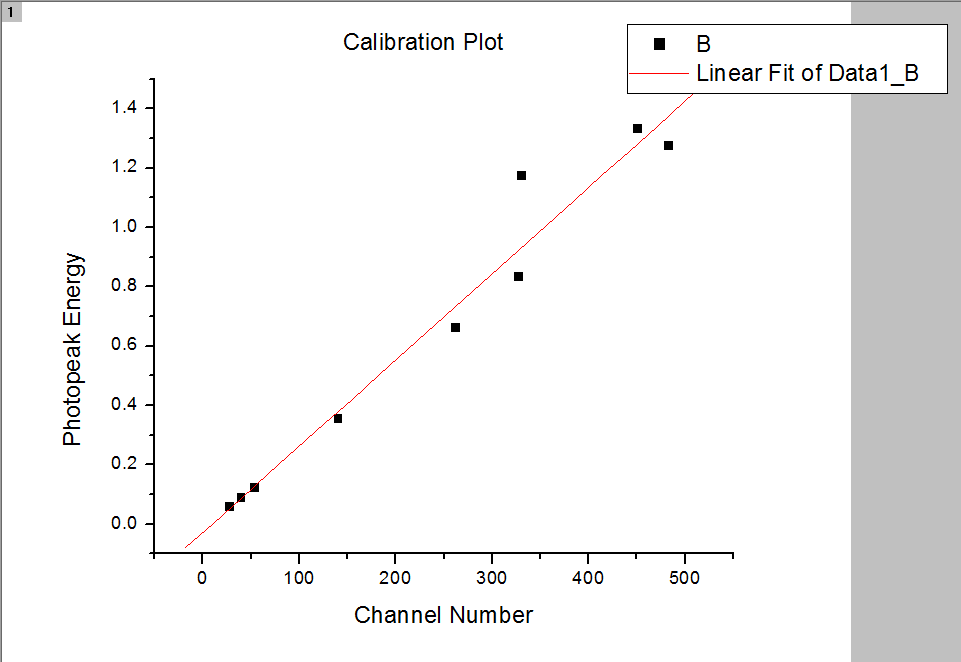
\includegraphics[width=.60\textwidth]{calibration_plot.png}
    \label{fig:calibration}
\end{figure}

Another very important step was to subtract the given background spectrum from our data before plotting it. As we found in lecture the background spectrum had been taken for twice as long as the other elements spectrum. Therefore, we had to divided the given background spectrum in half. We then subtracted these values from our given data. This effectively removed the background counts in our data and left only the real data. We then created our plots of the energy versus counts. 

\begin{figure}[H]
  \caption{The energy vs counts spectrum for americium-241.}
  \centering
    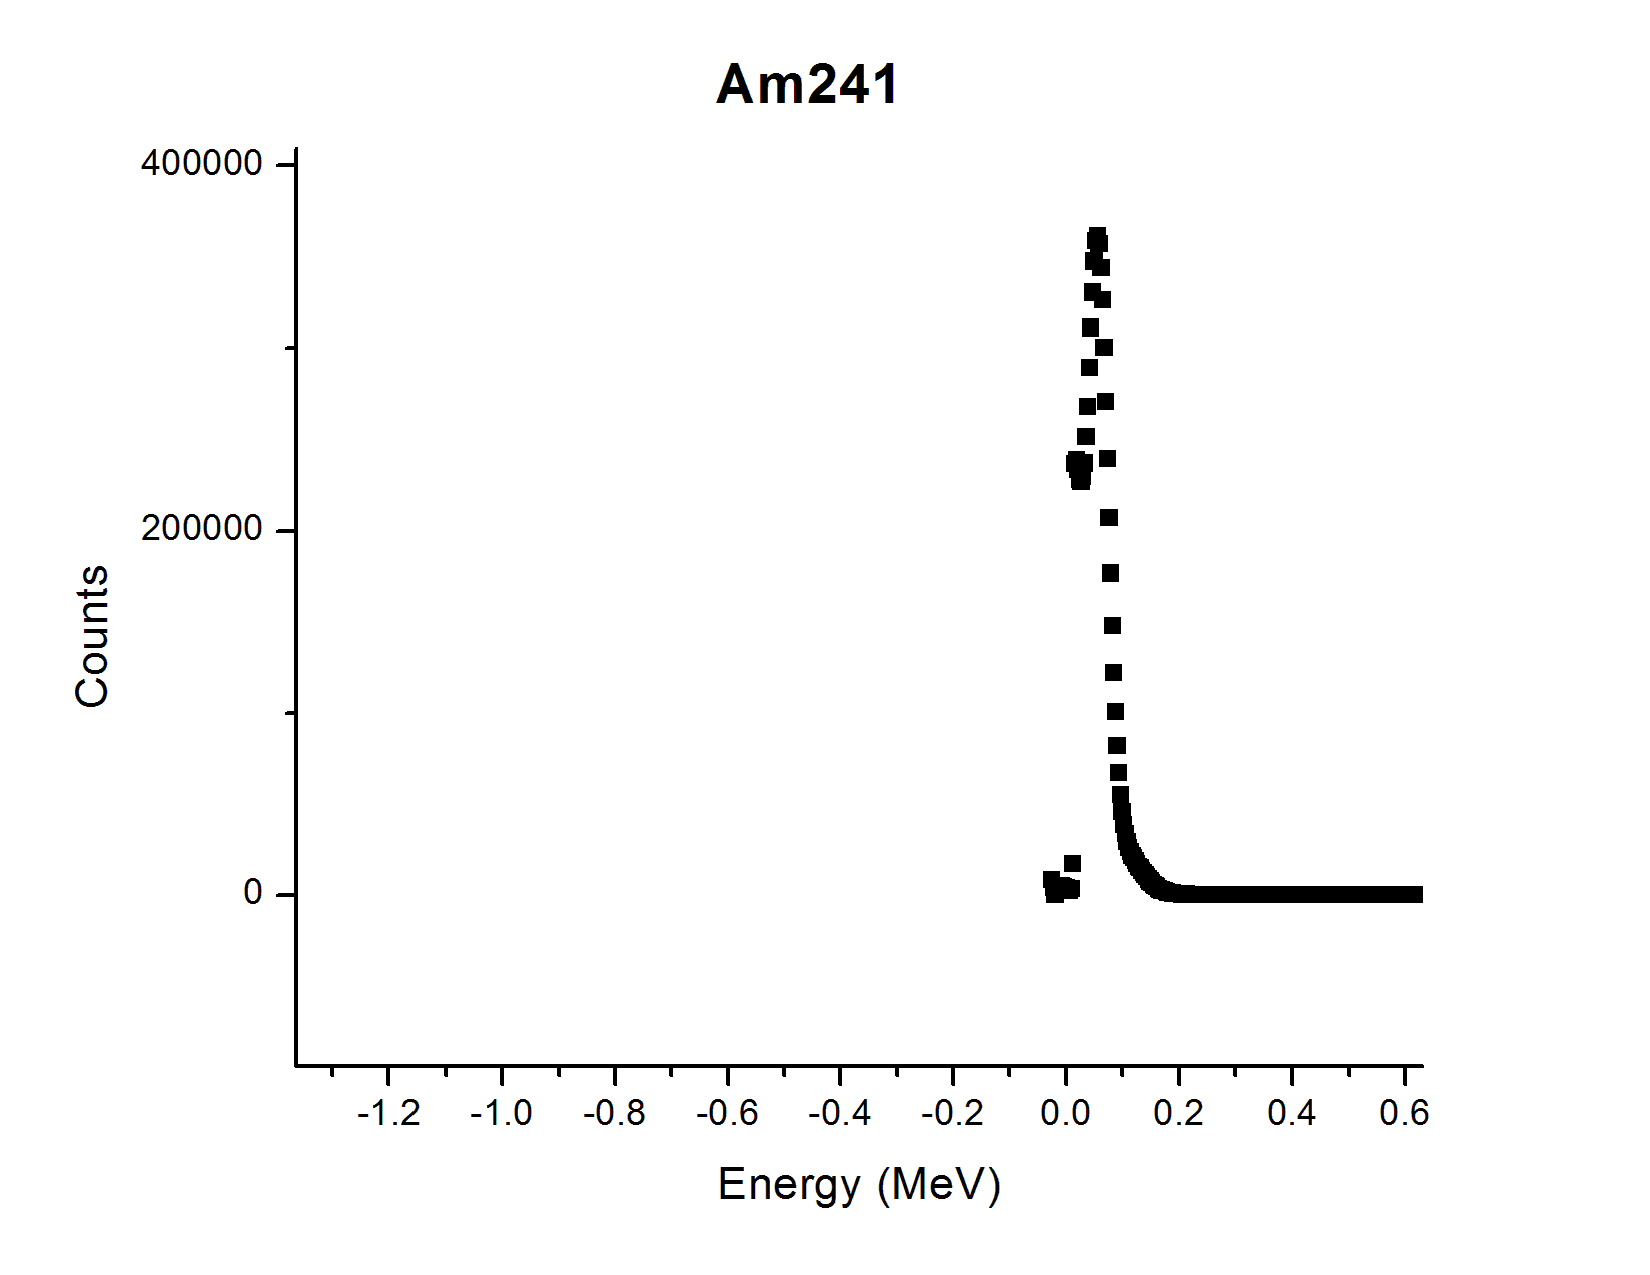
\includegraphics[width=.60\textwidth]{am241.JPG}
    \label{fig:am241}
\end{figure}

In this spectrum we don't see counts for any noteworthy energy. It would seem that this is more background radiation that wasn't subtracted off. The literature states that most common decay of Am-241 is an alpha decay which releases 5.388 MeV. Although the graphs scale doesn't go that high we didn't see this behavior before scaling down for this report. Clearly this must be a more rare alpha decay that didn't happen in the time the data was being collected. Perhaps poor data collection is suspect for the lack of counts too. 

\begin{figure}[H]
  \caption{The energy vs counts spectrum for barium-133.}
  \centering
    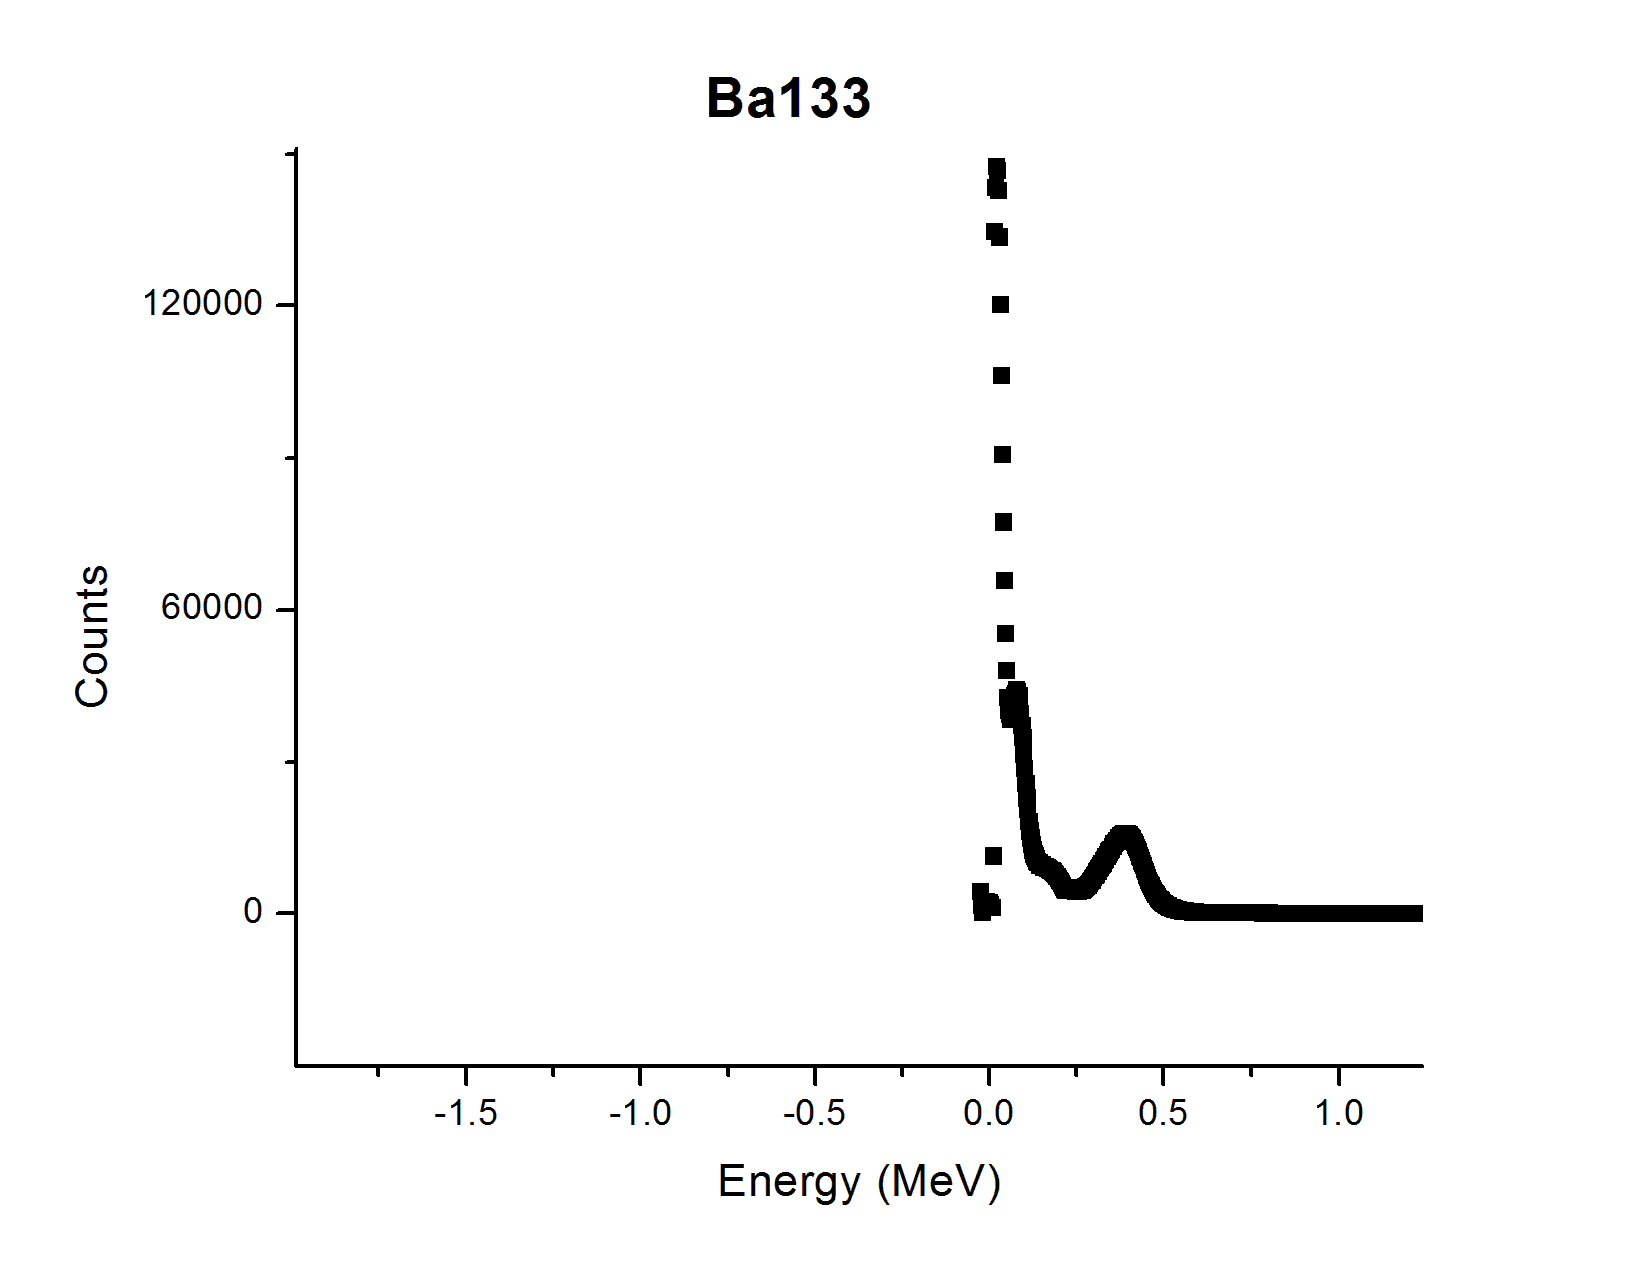
\includegraphics[width=.60\textwidth]{Ba133.JPG}
    \label{fig:ba133}
\end{figure}

In barium-133 we see a slight photo peak at about 0.356 MeV. Which exactly what we would expect. We also see a very slight Compton edge that trails off right before the photo peak which is what we would expect.  


\begin{figure}[H]
  \caption{The energy vs counts spectrum for cadmium-109.}
  \centering
    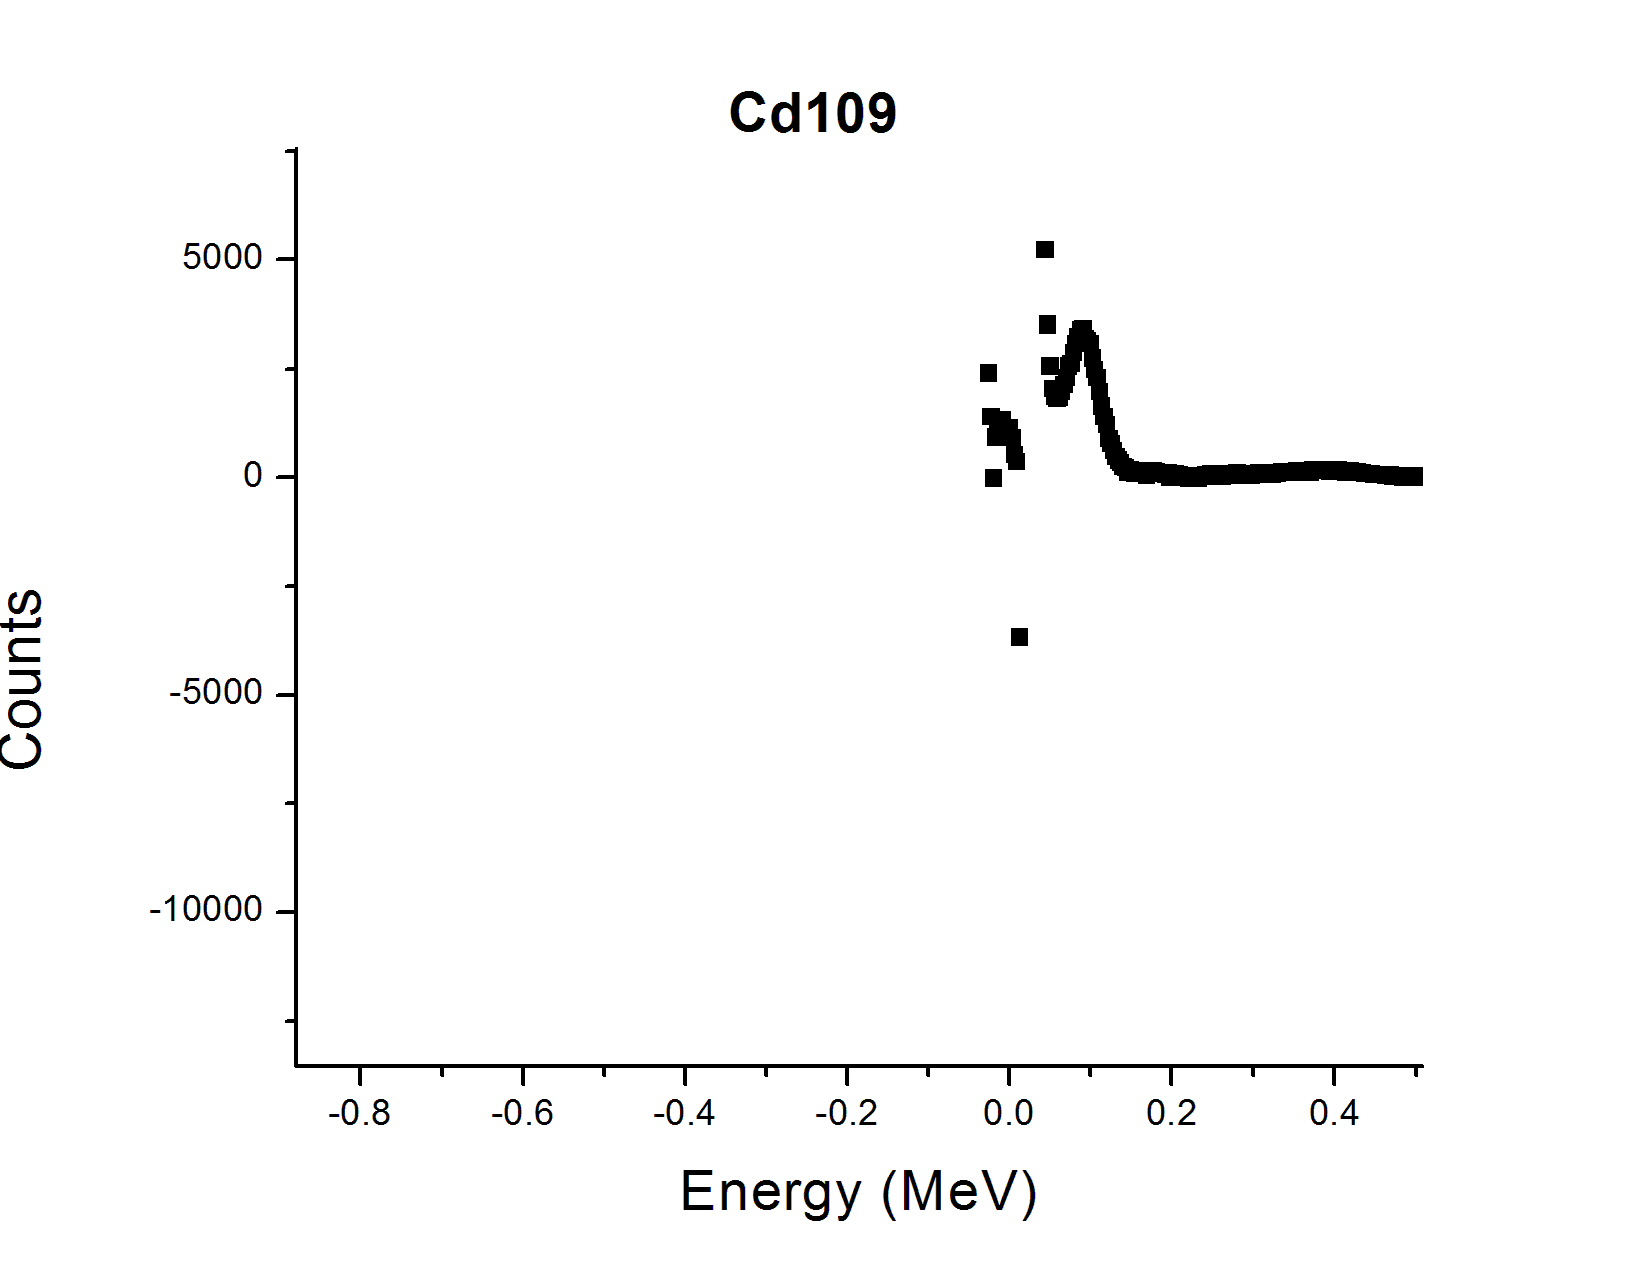
\includegraphics[width=.60\textwidth]{cd109.JPG}
    \label{fig:cd109}
\end{figure}

For cadmiu-109 we see a photo peak at around 0.09 MeV which is near what we would expect. We also see some high count values near zero MeV. We believe that this is background radiation that didn't get subtracted off, or it could be radiation from the apparatus itself. Both of these features are expected. 


\begin{figure}[H]
  \caption{The energy vs counts spectrum for cobalt-57.}
  \centering
    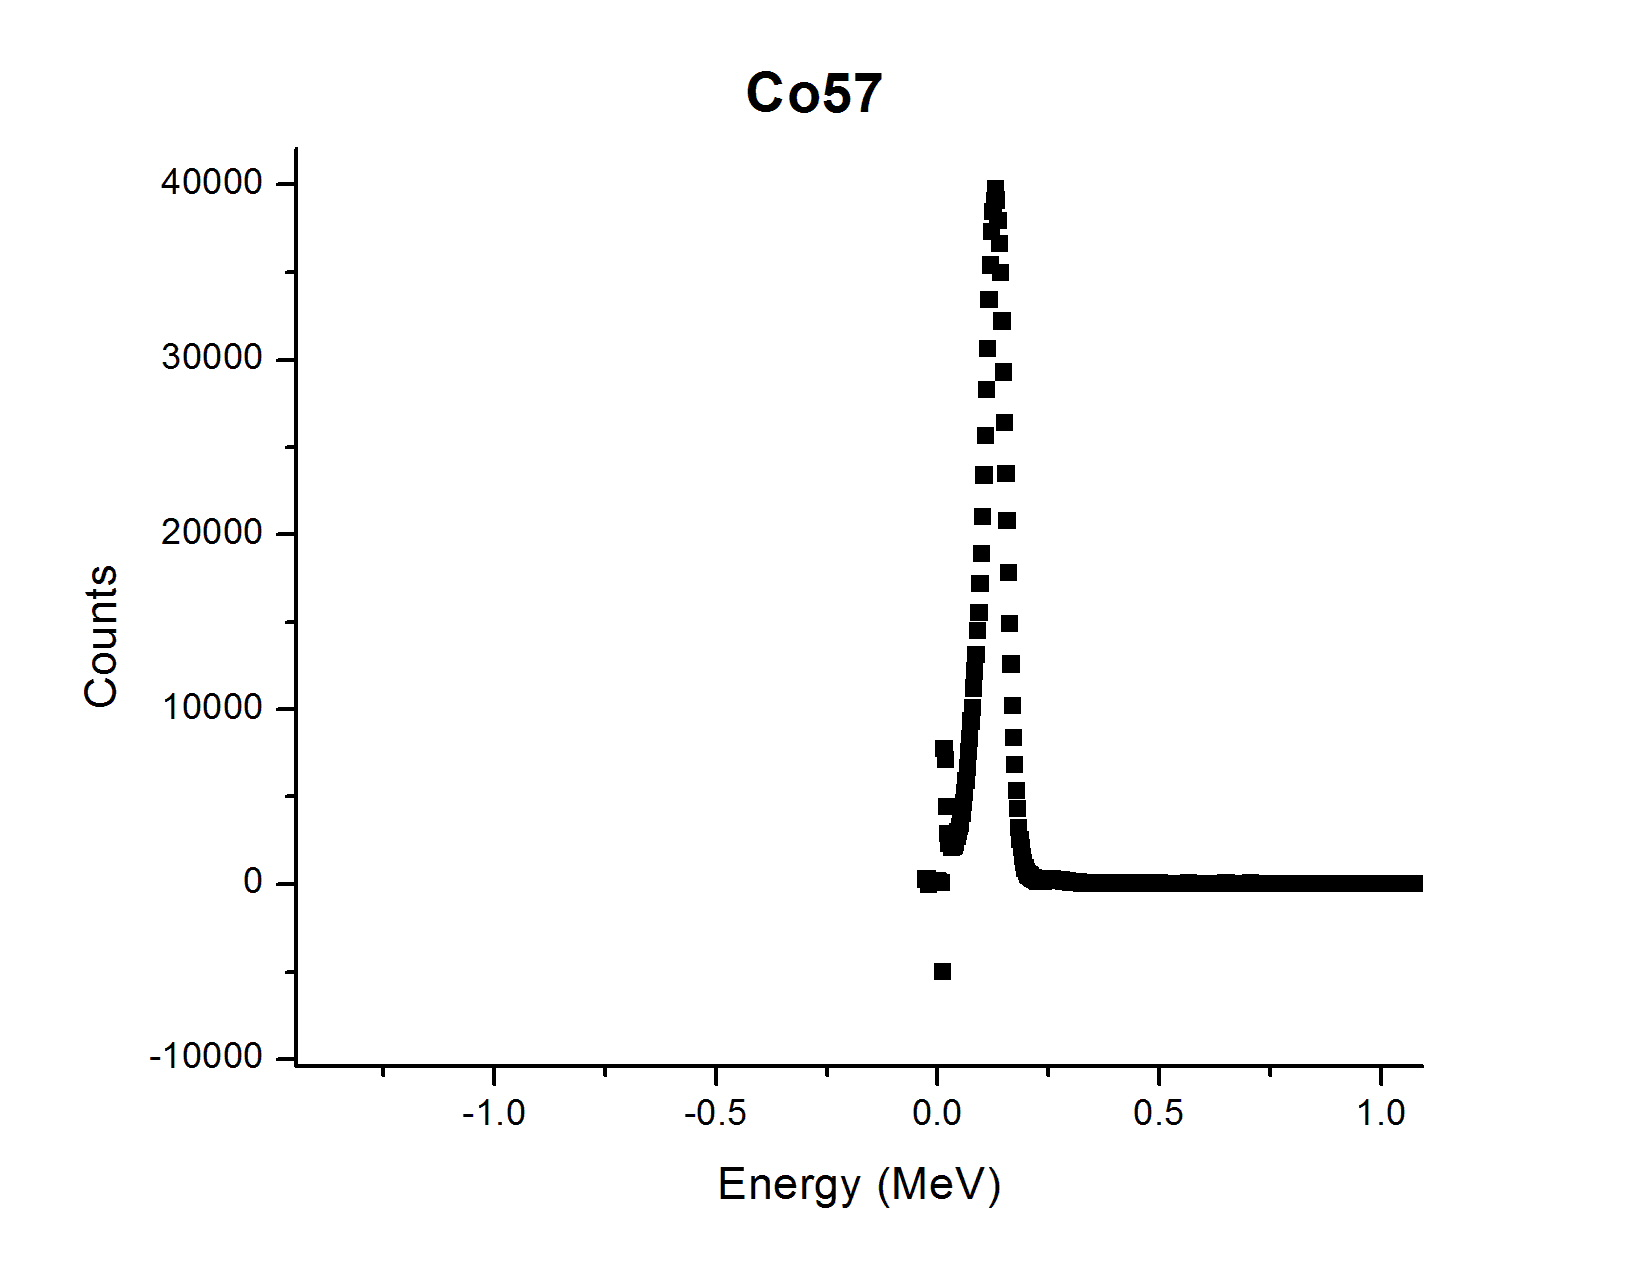
\includegraphics[width=.60\textwidth]{co57.JPG}
    \label{fig:co57}
\end{figure}

In cobalt 57 we can clearly see a photo peak that occurs near 0.122 MeV. This is what we would expect. We can also see a small amount of background radiation that didn't get subtracted off, or it could be radiation from the apparatus itself.

\begin{figure}[H]
  \caption{The energy vs counts spectrum for cobalt-60.}
  \centering
    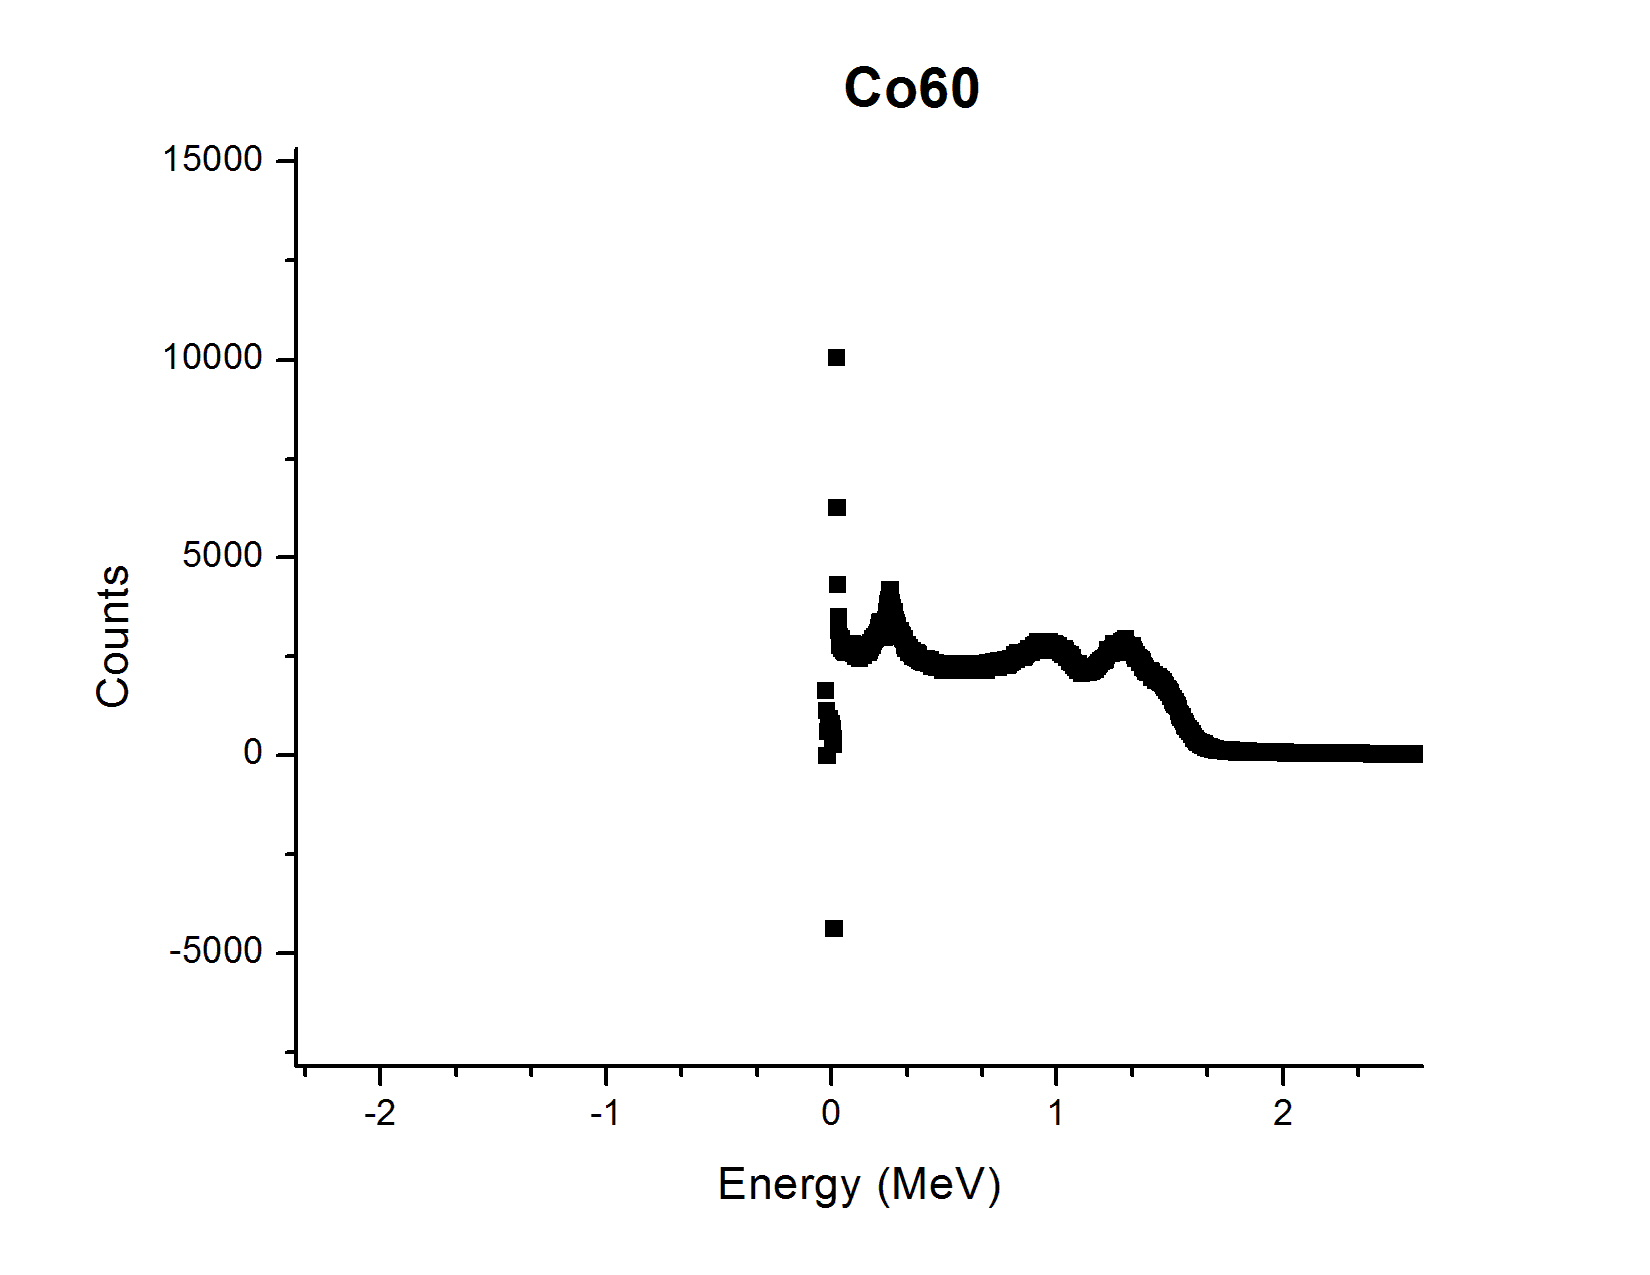
\includegraphics[width=.60\textwidth]{co60.JPG}
    \label{fig:co60}
\end{figure}

In cobalt 60 we can actually see two photo peaks. One is around 1.17 MeV, and the second is near 1.33 MeV. These two seem to almost morph together into a single peak. Each photo peak should have it's own corresponding Compton edge however it appears that they merge together and form a single Compton edge near 0.9 MeV. Each photo peak should also have it's own back scattered peak, but they once again seem to merge together into a single back scatter peak near 0.25 MeV. We also see some slight counts that could be from background radiation, or it could be radiation from the apparatus itself. It should be noted that the features would be more prominent and we would be able to distinguish between the two photo peaks and their corresponding features if we had great fidelity in our data. 

\begin{figure}[H]
  \caption{The energy vs counts spectrum for cesium-137.}
  \centering
    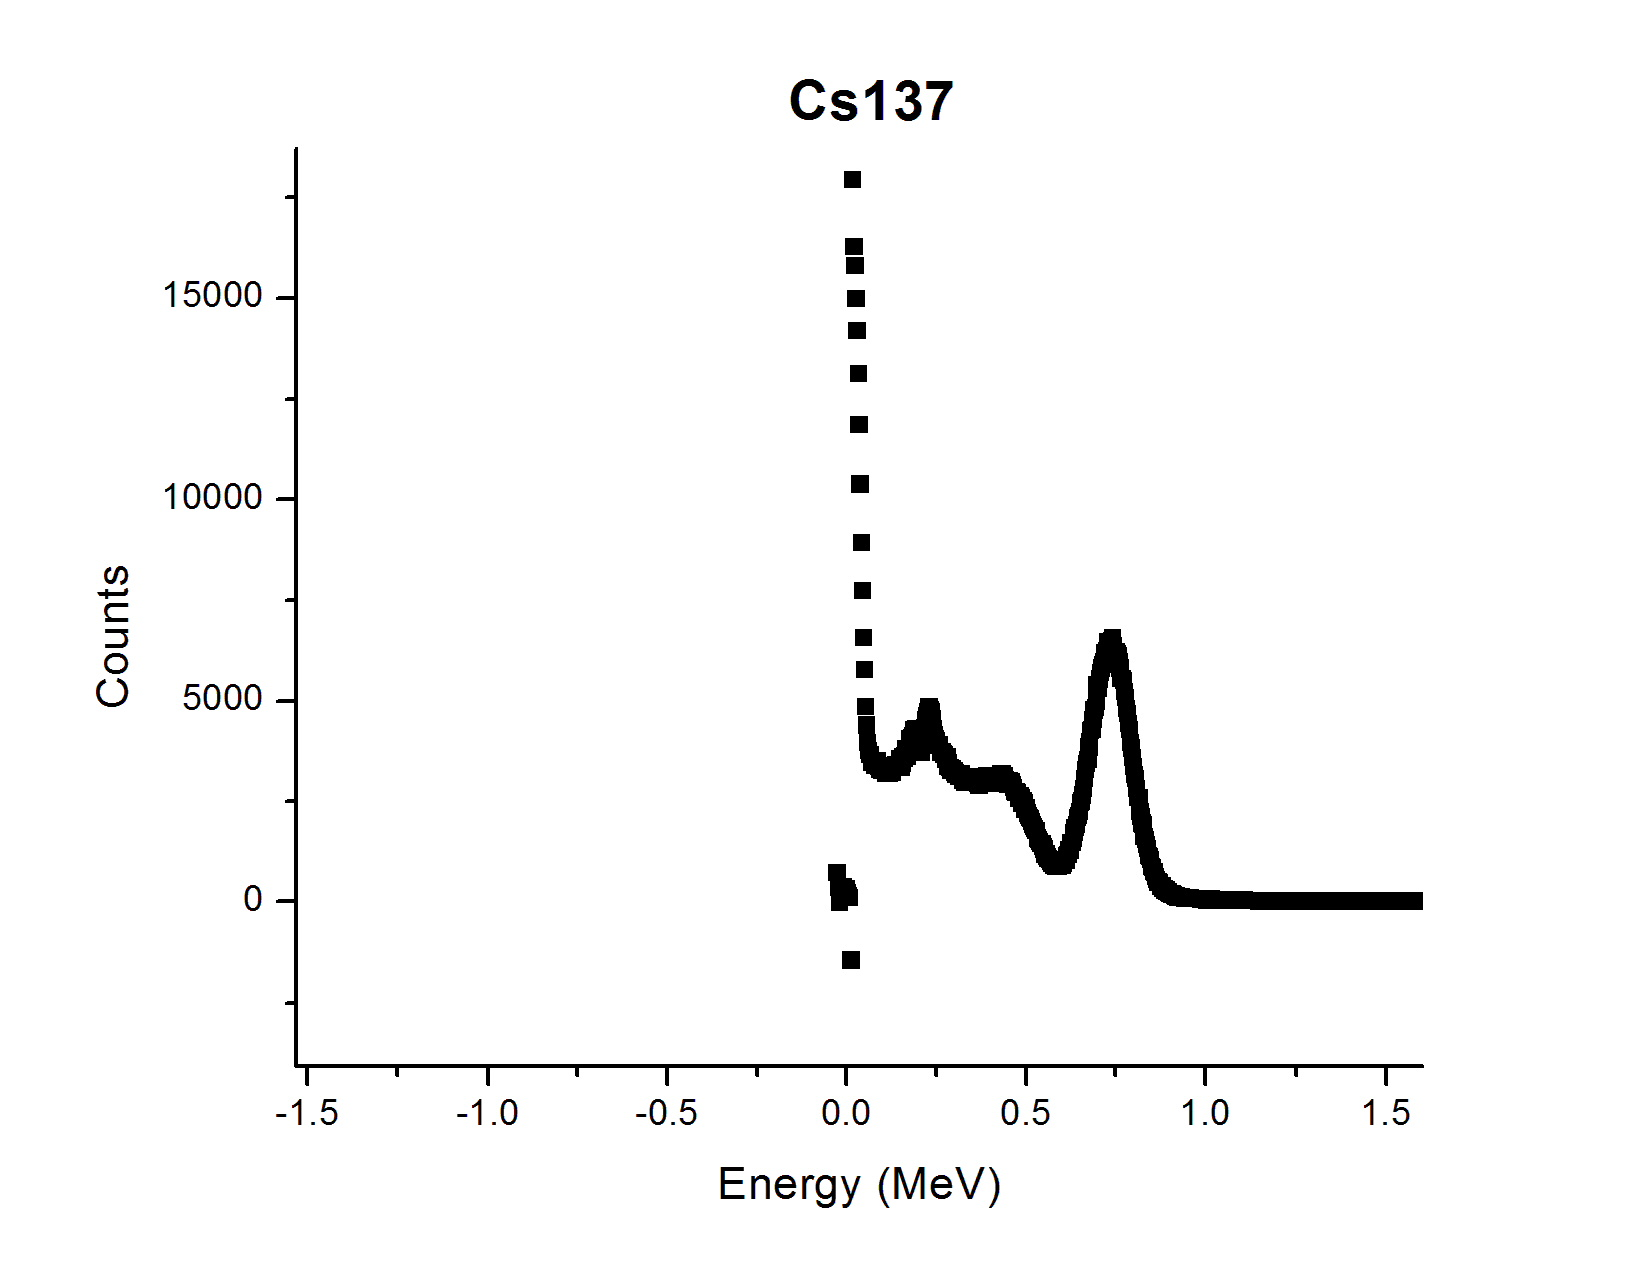
\includegraphics[width=.60\textwidth]{cs137.JPG}
    \label{fig:cs137}
\end{figure}

In cesium-137 we see a photo peak near 0.66 MeV which is about what we would expect. The photo peak is due to the photo electric effect. When a gamma ray hits the NaI crystal an electron is ripped off because the gamma ray energy is greater than the binding energy. The energy from the gamma ray is transferred to the electron and then we see the prominent peak at that energy. 

We also can see a Compton edge. The Compton edge is created by Compton scattering. The equation for this phenomena is 
\begin{equation}
\Delta \lambda = \frac{h}{m_e c} ( 1 - \cos \theta) 
\end{equation}

Where $\Delta\lambda$ is the change in wavelength from incoming gamma ray to the outgoing gamma ray after it has interacted with the electron. $h$ is Planck's constant, $m_e$ is the mass of an electron, $c$ is the speed of light, and $\theta$ is the angle between the outgoing gamma ray and the electron. 

When the gamma ray comes in and interacts with the electron it can transfer energy to it which depends on the angle that it came in from. From this equation we can see that the energy which is imparted to the electron can vary from $\theta=0$ to $\theta=180$. At when $\theta$ is 180 degrees it will get the maximum contribution of energy from the gamma ray (i.e. a ``head on" collision) and this is called the Compton edge. 

We can also see the back scatter peak near 0.4 MeV. This phenomena happens when the gamma ray hits the electron and the electron escapes and the new gamma ray is detected instead of the electron. This peak will be the difference between when the Compton edge ends and the central peak. The mathematical expression is 
$$ 
E_{\gamma'} = E_{\gamma} - E{e^-}
$$

Where $E_{\gamma}$ is the incoming gamma ray energy, $E{e^-}$ is the electron energy, and $E_{\gamma'}$ is the scattered gamma ray energy. What we detect in back scattering is the $E_{\gamma'}$. In our data the $E_{\gamma'}$ is 0.20 MeV so the back scattered peak should be at about 0.20 MeV which is what we find in the our experimental spectra. 

We also see some counts near zero energy. We believe that these could be left over background radiation that didn't get subtracted off, or radiation from the machine itself.  

\begin{figure}[H]
  \caption{The energy vs counts spectrum for manganese-54.}
  \centering
    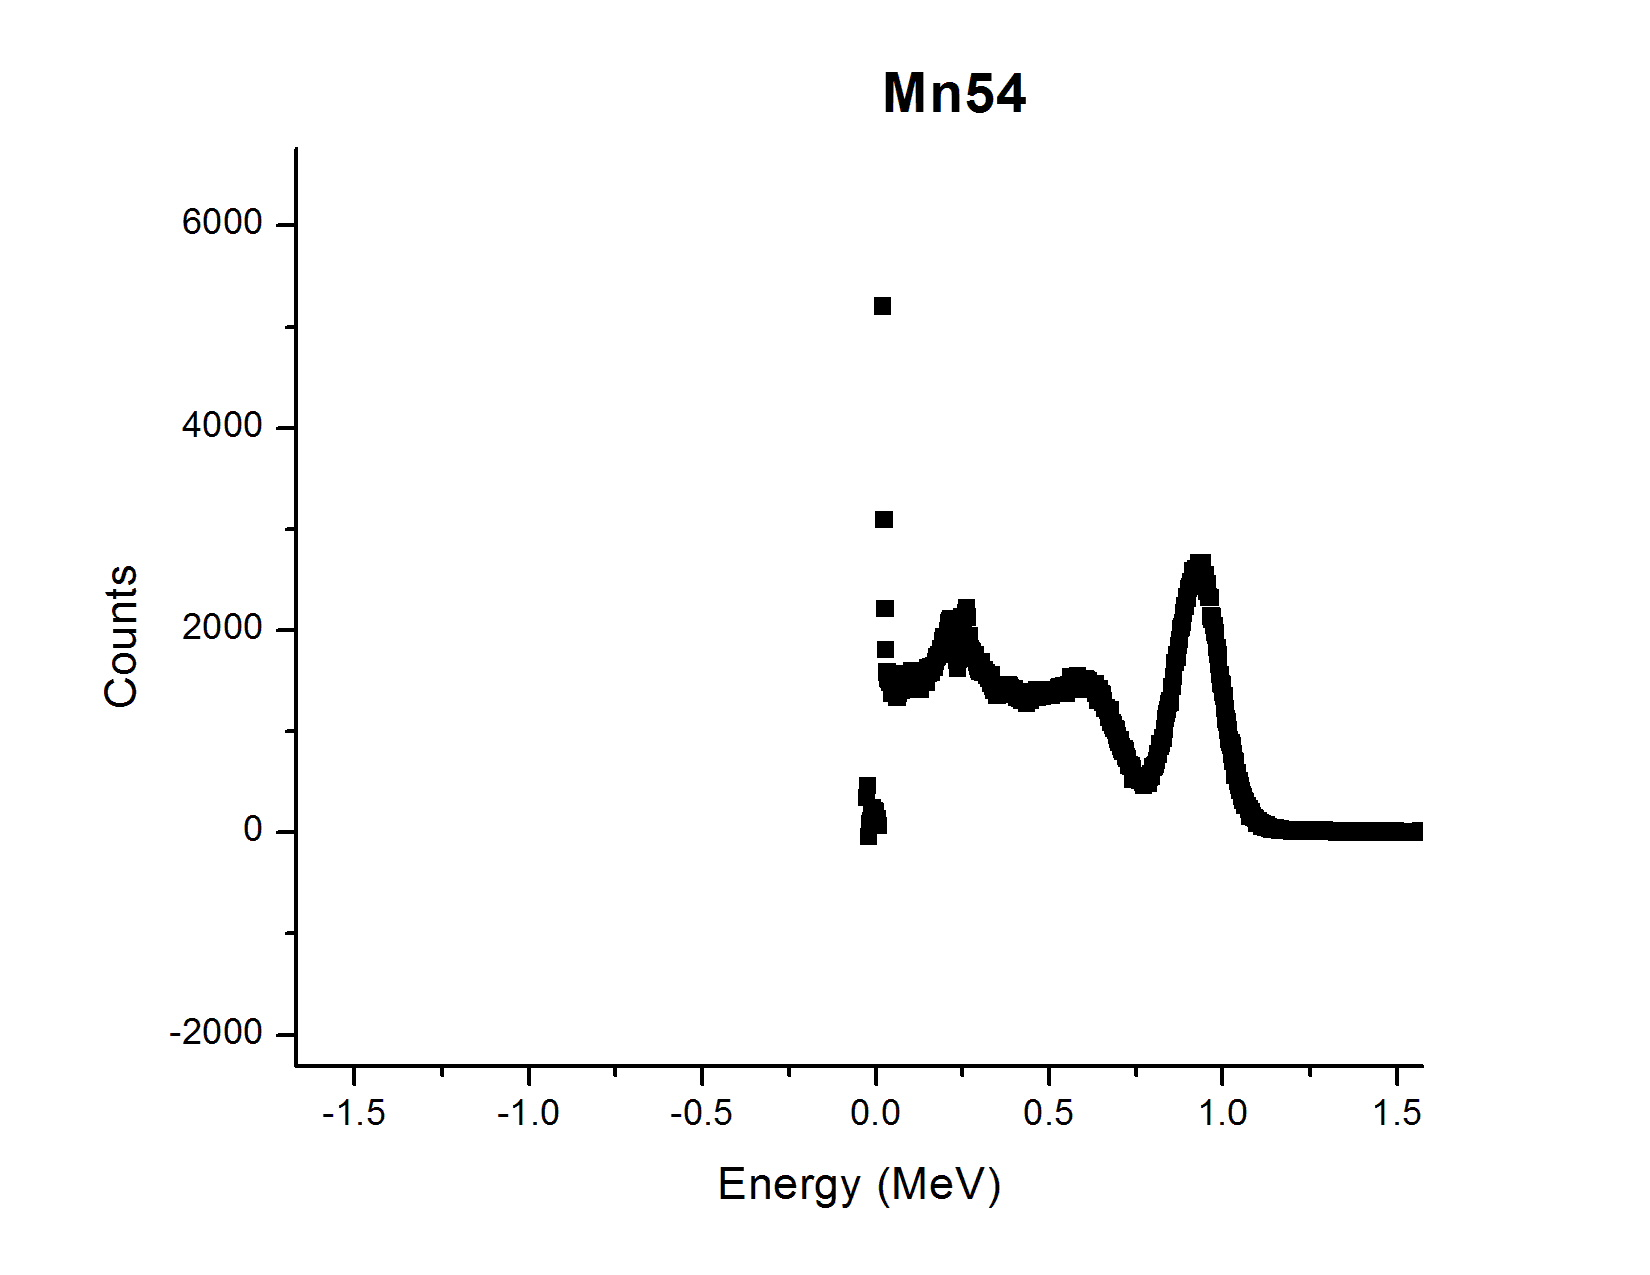
\includegraphics[width=.60\textwidth]{mn54.JPG}
    \label{fig:mn54}
\end{figure}

In manganese-54 we can see a photo peak near 0.83 MeV which is what we would expect, and also the Compton edge that ends near 0.60 MeV. Both of these we would expect when we compare with the literature. 


\begin{figure}[H]
  \caption{The energy vs counts spectrum for sodium-22.}
  \centering
    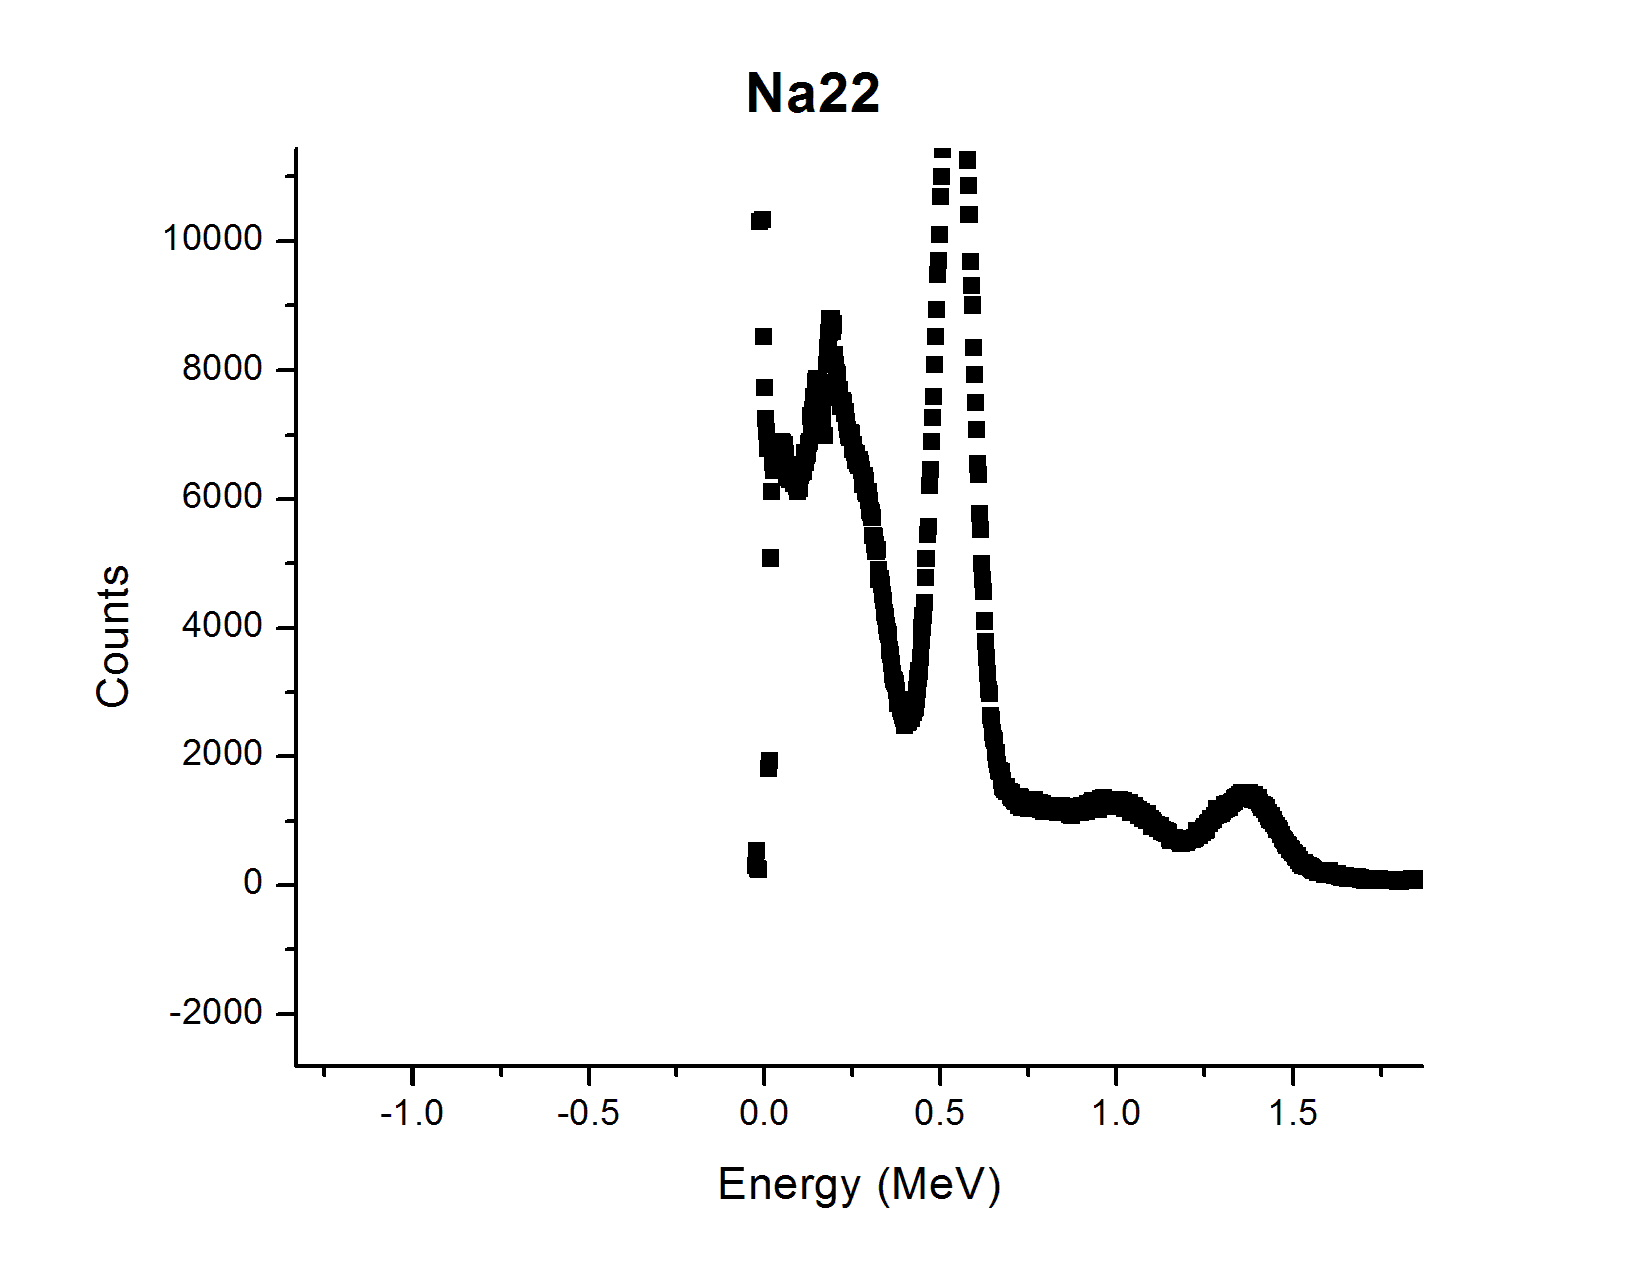
\includegraphics[width=.60\textwidth]{na22.JPG}
    \label{fig:na22}
\end{figure}

In sodium-22 we can see the photo peak at 1.27 MeV and also the Compton edge. We can also note the pear at 0.5 MeV which is due to pair production. Sodium-22 is special because it is a positron emitter. We also see a beta peak at around 0.2 MeV. All of these are as expected with our given theory. 



\section*{Results and Conclusions}

In this experiment looked at the gamma spectrum for numerous radioactive elements. We were able to look at their spectrum and determine the various mechanisms that theory predicts. We were also then able to compare with other experimental data available to see how good our data was. 

To find the the energy of an electron we can use the equation for the Compton effect and the energies of $E_{\gamma}$ and $E_{\gamma'}$ to find the rest mass of an electron. We can use our modified Compton effect equation 

\begin{equation}
E_{\gamma'} = \frac{E_{\gamma}}{1 + \frac{E_{\gamma}}{m_e c^2}(1 - \cos(\theta))}
\end{equation}

If we set $\theta = 180$ then we get 

\begin{equation}
E_{\gamma'} = \frac{E_{\gamma}}{1 + \frac{2E_{\gamma}}{m_e c^2}}
\end{equation}

We can then solve this for the mass of the electron $m_e$ and plug in $E_{\gamma}$ as the photo peak of a sample and $E_{gamma'}$ as the energy at the Compton edge. We find these values for cesium 137 to be 0.66 MeV and 0.45 MeV. When we plug these values in we find the rest mass of the electron to be 7.33\e{-24} kg. This is nowhere near the value of 9.109\e{-30} kg that we would expect. So, either we have bad data, or we did the calculation wrong. 


\begin{figure}[H]
  \caption{The energy vs counts spectrum for an unknown sample.}
  \centering
    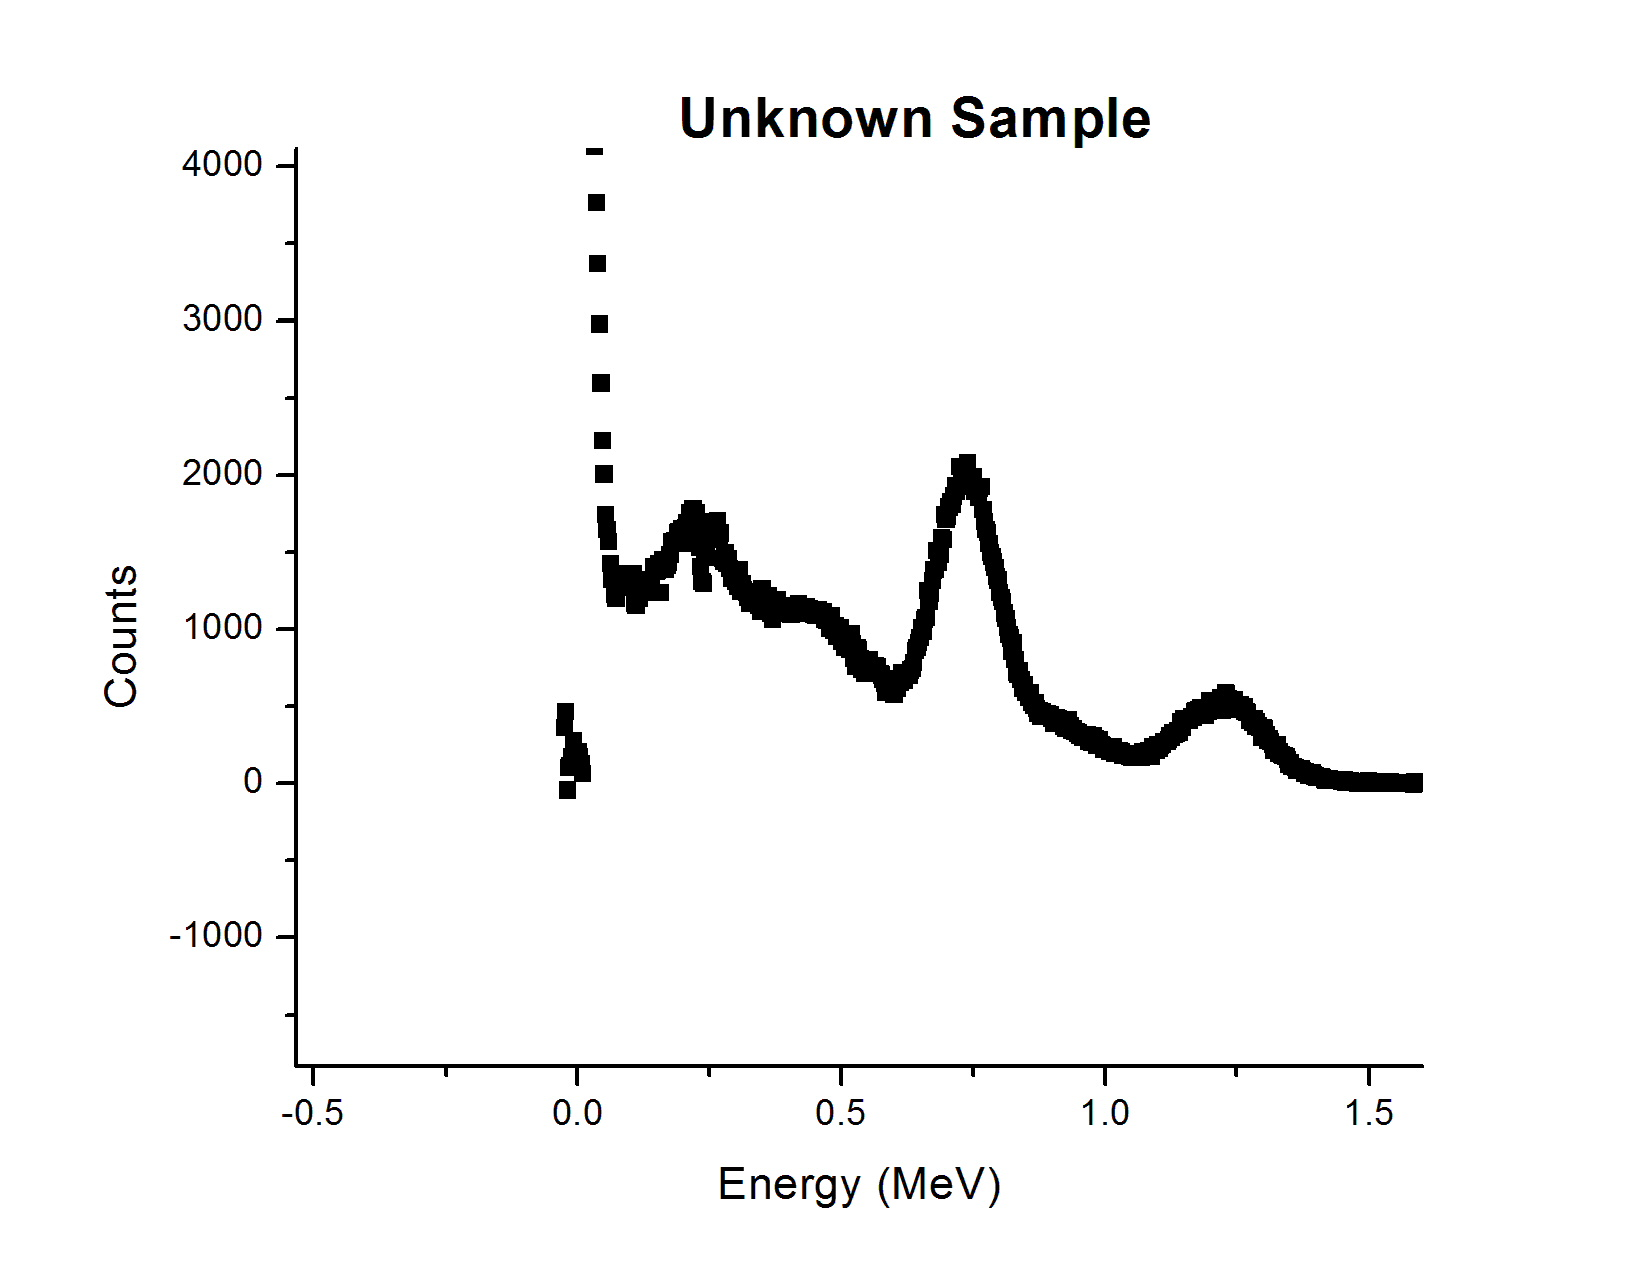
\includegraphics[width=.60\textwidth]{unknown_sample.JPG}
    \label{fig:unknown_sample}
\end{figure}

In our unknown sample we notice two prominent photo peaks. We were told that the sample had zinc in it. We found that zinc-60 has a prominent decay at 0.67 MeV. So we believe that's what that photo peak is from. We also believe the other peak higher in energy is due to a cobalt-60 whose spectrum has been pushed together. If you look closely you can make out two very faint peaks. Since cobalt-60 has two peaks near this energy of 1.2 MeV we are lead to believe that those peaks are from it. So, we believe it is a zinc-60 and cobalt-60 sample. 

In order to determine the resolution of the detector we used a measure of full width half maximum on two different photo peaks. Since the photo peaks are approximately Gaussian we can use the equation 
\begin{equation}
 \mathrm{FWHM} =   2\sqrt{2 \ln 2 } \; \sigma \approx 2.355 \; \sigma.
\end{equation}

So we took our two full width at half maximum values and took an average and we found it to be 0.15 MeV. 

\end{document}